\subsection{Algoritmo genético}
Para esta práctica se desarrolló un algoritmo genético que se apega al proceso mostrado en la Figura \ref{fig:AG}.

\begin{figure}[htbp]
	\centering
	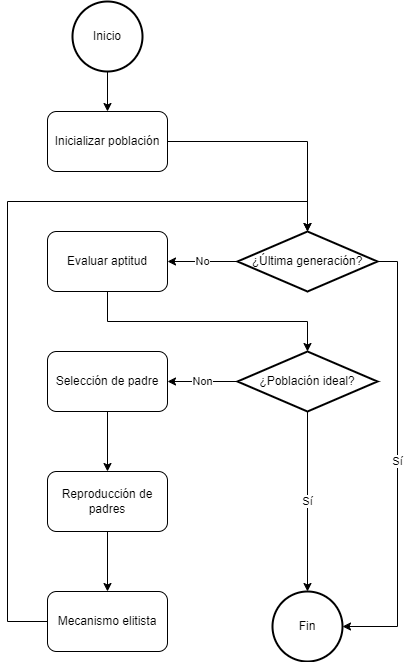
\includegraphics[width=0.5\textwidth]{algoritmo_genetico_proceso}
	\caption{Diagrama de flujo del algoritmo genético implementado.}
	\label{fig:AG}
\end{figure}

Para llevar a cabo dicho proceso, se optó por utilizar el lenguaje de programación Python, donde se diseñaron métodos genéricos para realizar los procesos de generación de población, evaluación de aptitud, selección de individuos, reproducción de individuos, mutación y mecanismos elitistas.

\subsection{Implementación en Python}

\subsubsection{Inicializador de población}
\inputminted[linenos=true, fontsize=\scriptsize]{Python}{../../utils/population.py}

\subsubsection{Evaluación de individuos}
\inputminted[linenos=true, fontsize=\scriptsize]{Python}{../cities.py}

\inputminted[linenos=true, fontsize=\scriptsize]{Python}{../distance_helper.py}

\inputminted[linenos=true, fontsize=\scriptsize]{Python}{../../utils/aptitude.py}

\subsubsection{Selección de parejas}
\inputminted[linenos=true, fontsize=\scriptsize]{Python}{../../utils/selection.py}

\subsubsection{Reproducción de individuos}
\inputminted[linenos=true, fontsize=\scriptsize]{Python}{../../utils/crossover.py}

\subsubsection{Mutación}
\inputminted[linenos=true, fontsize=\scriptsize]{Python}{../../utils/mutation.py}

\subsubsection{Algoritmo completo}
\inputminted[linenos=true, fontsize=\scriptsize]{Python}{../P2_EnriqueMenaCamilo.py}

\subsection{Pruebas realizadas}
Se implementaron un total de 2 mecanismos de selección, 2 mecanismos de cruza, 2 mecanismos de mutación y 1 mecanismo elitista. Se optó por realizar una combinación de todos los mecanismos de selección con todos los mecanismos de cruza, intercalando los mecanismos de mutación. Las combinaciones resultantes fueron:

\begin{itemize}
	\item Algoritmo 1: Selección Ruleta + PMx + Insert Mutation + 100 individuos.
	\item Algoritmo 2: Selección Ruleta + Cx + Inverse Mutation + 250 individuos.
	\item Algoritmo 3: Selección Torneo + PMx + Insert Mutation + 500 individuos.
	\item Algoritmo 4: Selección Torneo + Cx + Inverse Mutation + 1000 individuos.
\end{itemize}

Cabe destacar que, dado que solamente se implementó 1 mecanismo elitista, este fue aplicado a todos los algoritmos por igual. También es importante mencionar que se implementó 1 criterio de paro híbrido:

\begin{itemize}
	\item Número de generaciones. Se estableció un límite de 10 generaciones para todos los algoritmos.
	\item Término por $\delta$. Se estableció un valor $\delta=1000$ con un máximo de 50 generaciones.
\end{itemize}
